\documentclass{beamer}  

\usetheme{Berlin}
\usetheme{boxes}
\usepackage[spanish]{babel}
\usepackage[T1]{fontenc}
\usepackage[utf8]{inputenc}
\usepackage{graphicx}
\usepackage{tikz}
\usepackage{etex}

\title{Nucleotide String Library}
\author{~Delgado Quesada Juan Jos\'e (B42250)\\
Fallas Pizarro Jose Ariel (B42481)\\
Martinez Garcia David (B34019)
}

\institute[Universidad de Costa Rica] 
{
  Escuela de Ingenier\'ia El\'ectrica\\
  Facultad de Ingenier\'ia \\
  Universidad de Costa Rica}

\date{Proyecto Grupal, II Semestre, 2015 \\
		IE-0217}

\AtBeginSubsection[]
{
  \begin{frame}<beamer>{Outline}
    \tableofcontents[currentsection,currentsubsection]
  \end{frame}
}

\begin{document}

\begin{frame}
  \titlepage
\end{frame}
\begin{frame}
\frametitle{Nucleotide String Library}
\textbf{\large{Justificación}}
  	\begin{figure}
		
\includegraphics[width=0.8in]{CIB.png}
	\end{figure}
 	\begin{figure}
		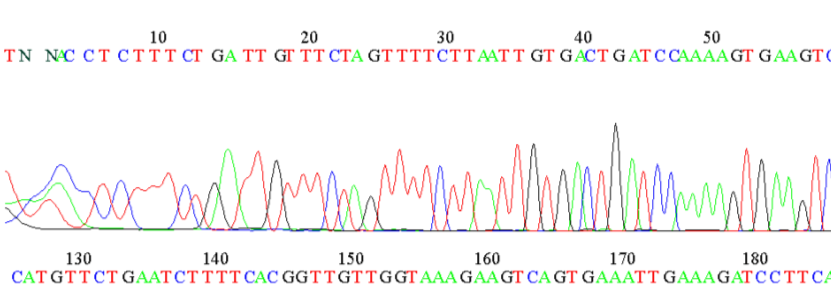
\includegraphics[width=4.0in]{muestra.png}
	\end{figure}
\end{frame}

\begin{frame}
\frametitle{Nucleotide String Library}
\textbf{\large{Objetivo General}}
\begin{itemize}
\item Implementar una librer\'ia en C++ que facilite el trabajo y procesamiento de secuencias de bases nitrogenadas y a su vez permita trabajar con bases de datos de cadenas de bases nitrogenadas \textbf{(BLAST)}.
\end{itemize}
 	\begin{figure}
		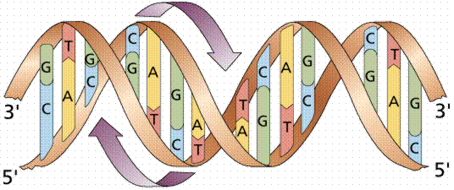
\includegraphics[width=2.0in]{ADN.jpg}
	\end{figure}
\end{frame}

\begin{frame}
\frametitle{Nucleotide String Library}
\textbf{\large{Objetivo específico}}
\begin{itemize}
\item Diseñar y estructurar las clases necesarias, que conformaran la Libreria para el manejo de bases nitrogenadas, con sus respectivas funciones.
\end{itemize}
\begin{figure}
		
\includegraphics[width=1.5in]{C.png}
\end{figure}
\end{frame}

\begin{frame}
\frametitle{Nucleotide String Library}
\textbf{\large{Clase NucleoString :}}
\begin{itemize}
\item{getfasta, headerret}
\item{chainret, cut}
\item{transcript, complement}
\end{itemize}
\begin{figure}
		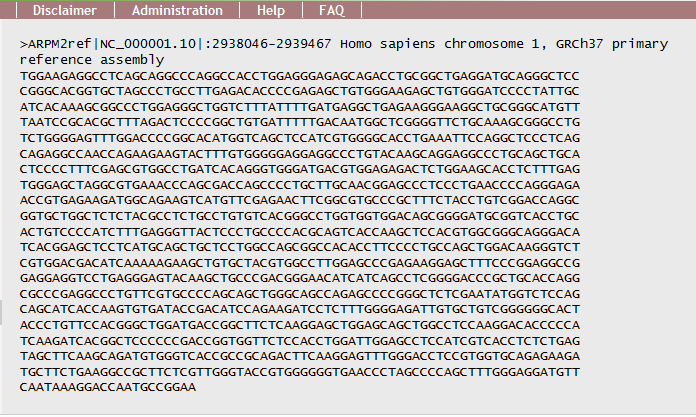
\includegraphics[width=3.0in]{fasta.png}
\end{figure}
\end{frame}

\begin{frame}
\frametitle{Nucleotide String Library}
\textbf{\large{Clase Helix :}}
\begin{figure}
		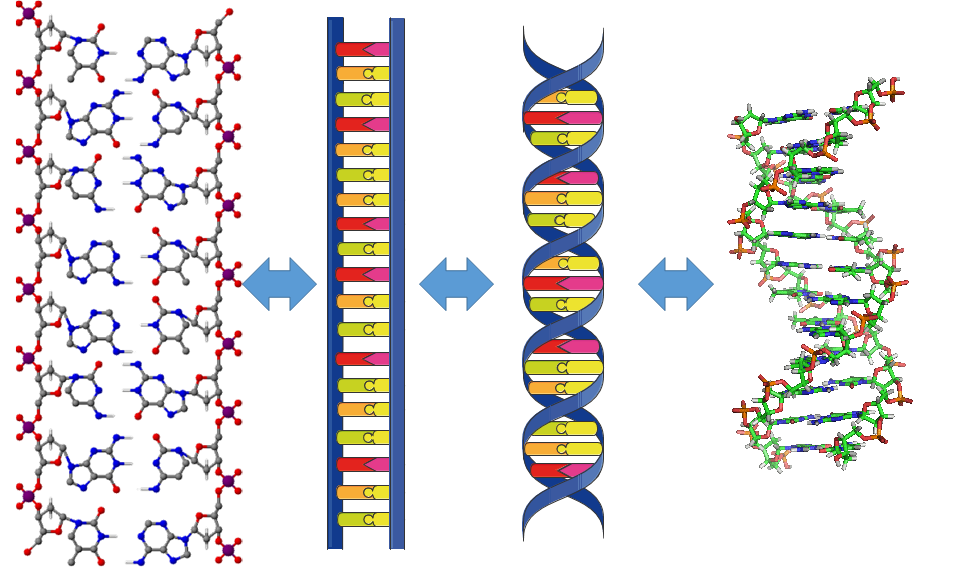
\includegraphics[width=3.0in]{ADN.png}
\end{figure}
\end{frame}

\begin{frame}
\frametitle{Nucleotide String Library}
\textbf{\large{Clase NucleoString :}}
\begin{itemize}
\item{getfasta, headerret}
\item{chainret, cut}
\item{transcript, complement}
\end{itemize}
\begin{figure}
		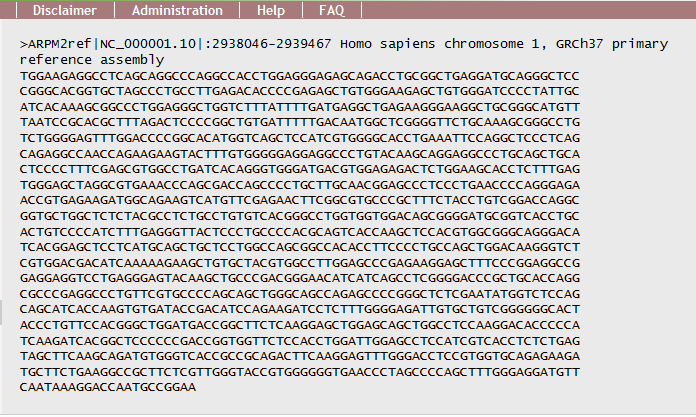
\includegraphics[width=3.0in]{fasta.png}
\end{figure}
\end{frame}

\begin{frame}
\frametitle{Nucleotide String Library}
\textbf{\large{Clase Management}}
\begin{itemize}
\item{CRef<IQueryFactory> FetchQuerySequence(NucleoString<ARN>);}
\item{CSearchDatabase FetchBlastNDataBases(void);}
\item{CRef<CBlastOptionsHandle> FetchOptionsBlastN(void);}
\end{itemize}
\begin{figure}
		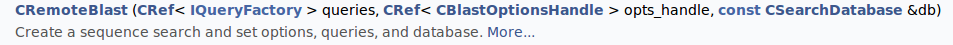
\includegraphics[width=4.7in]{remote.png}
\end{figure}
\end{frame}

\begin{frame}
\frametitle{Nucleotide String Library}
\textbf{\large{Objetivo específico}}
\begin{itemize}
\item Desarrollar una aplicación que permita poner en práctica las funciones y clases perteneciente a la libreria para el manejo de bases nitrogenadas.
\end{itemize}
\begin{figure}
		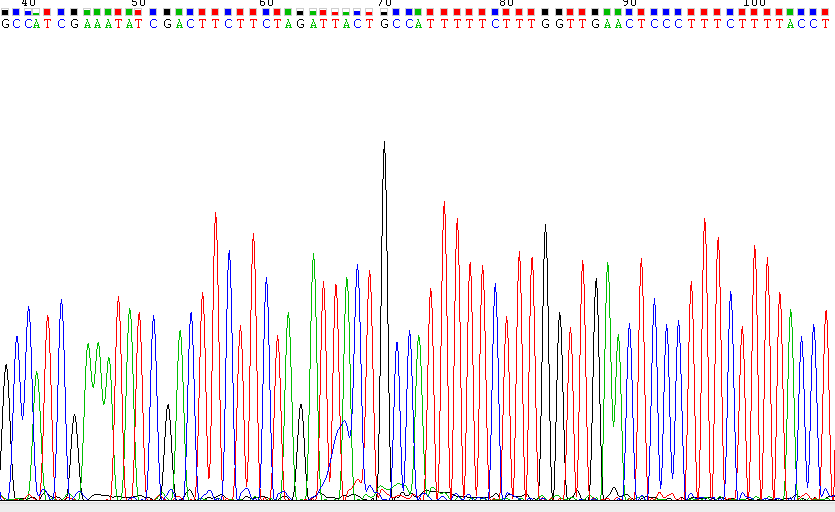
\includegraphics[width=3.5in]{2.png}
\end{figure}
\end{frame}

\begin{frame}
\frametitle{Nucleotide String Library}
\textbf{\large{Objetivo específico}}
\begin{itemize}
\item Poner en práctica los conocimientos vistos en el curso de Estructuras Abstractas de Datos y Algoritmos para Ingeniería como lo son: el uso de Templates y el análisis de la efectividad.
\end{itemize}
\begin{figure}
		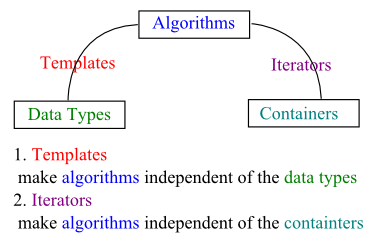
\includegraphics[width=3.0in]{templates.png}
\end{figure}
\end{frame}

\begin{frame}
\frametitle{Nucleotide String Library}
\textbf{\large{GRACIAS!!}}
\end{frame}



\end{document}